\subsection{Synaptic spine dynamics} \label{sec:spine-model}
\textbf{The model:} Synaptic spines are protrusions from dendrites and form contacts with chemically connected cells. Examples of 3D-reconstructed spines are shown in Fig.~\ref{fig:spine-types}. The spine-interior often contains an organelle, the spine apparatus (SA), which is a continuous extension of the endoplasmic reticulum (ER) in the dendrite. The ER is a multifunctional intracellular organelle of a neuron,
which consists of a complex three-dimensional network of connected endomembrane
tubules, stacks and cisternae, is involved in various ion exchange processes,
%cf. Fig.~\ref{fig:schematics},
\cite{Breit2018}, and ultimately responsible for synaptic plasticity. The SA and ER membrane harbors calcium exchangers that operate between the cytosol and ER domains. Typically, these are IP3-receptors, Ryanodine-receptors, and SERCA pumps. 
%(see Fig.~\ref{fig:schematics}A). 
On the plasma membrane additional calcium exchangers operate between the extra- and intracellular space, namely Plasma Membrane Calcium Pumps (PMCA), sodium-calcium-exchangers (NCX) {and voltage dependent calcium channels (VDCCs)}. 
The relevant quantities that need to be tracked on the 4D space/time cylinder are intracellular calcium $\textrm{Ca}^{2+}$, the molecule $\textrm{IP}_3$, which activates IP3-receptors together with $\textrm{Ca}^{2+}$, and mobile buffers, such as calbindin-D28k. One can define the following diffusion-reaction system first with the interaction between cytosolic $\textrm{Ca}^{2+}$ calbindin-$\textrm{D}_{28k}$ (CalB) is described by
\begin{align}
  \mathrm{Ca}^{2+}+\mathrm{CalB}\;\xrightleftharpoons
  [\kappa_{b}^{-}]{\kappa_{b}^{+}}\;[\mathrm{CalBCa}^{2+}].
\end{align}
\noindent The full domain equations for cytosolic calcium and calbindin-$\textrm{D}_{28k}$ are thus given by
\begin{align}
  \delT{\ccyt} & \;=\; \nabla \cdot \left( D_{c} \nabla \ccyt \right) \;+\;
    \left(\kappa_{b}^{-}\left(b^{\mathrm{tot}}-b\right)
        -\kappa_{b}^{+}\:b\:\ccyt\right), \label{eq:ccyt}\\
  \delT{b} & \;=\; \nabla \cdot \left( D_{b} \nabla b \right) \;+\;
    \left(\kappa_{b}^{-}\left(b^{\mathrm{tot}}-b\right)
        -\kappa_{b}^{+}\:b\:\ccyt\right)  \label{eq:buff}
\end{align}
\noindent Exponential IP\textsubscript{3} decay towards a basal IP\textsubscript{3} concentration
$p^r$ in the cytosolic space is modeled by a reaction term that is added to the
IP\textsubscript{3} diffusion equation, leading to the diffusion-reaction equation
\begin{align}
  \delT{\ip3} & \;=\; D_p\Delta\ip3 \;-\; \kappa_{\ip3}\left(\ip3-{\ip3}^{r}\right)
\end{align}
for IP\textsubscript{3} in the cytosolic domain.
Endoplasmic Ca\textsuperscript{2+} dynamics are modeled by simple diffusion
\begin{align}
  \delT{\cer} & \;=\; D_{c}\Delta\cer
\end{align}
in the endoplasmic domain. Nonlinear Neumann boundary conditions, which are defined by the calcium channel and pump models. 
%depicted in Fig.~\ref{fig:schematics}, complete the model. 
For the specifics of the ordinary differential equations that define PMCA, NCX, RyR, and SERCA pumps we refer to \cite{Breit2018b}. {The VDCCs are plasma membrane channels which release calcium into the cytosol once a voltage is applied to the plasma membrane. The flux equations for VDCCs are given by
\begin{equation}
	j_{vdcc}=G(V,t)F(V,\Delta [\textrm{Ca}^{2+}])
\end{equation}
where $G$ is the gating function and $F$ is the flux function (\cite{BorgGraham}). 
%Both depend on the voltage at the channel at a  particular time $t$. For the function $F$, the input value $\Delta [\textrm{Ca}^{2+}]$ is the difference in the internal and external ion concentration $\Delta [\textrm{Ca}^{2+}]=[\textrm{Ca}^{2+}]_i-[\textrm{Ca}^{2+}]_o$, the precise function of $F$ is given in \cite{BorgGraham}. 
%The gating function $G$ is described by a finite product $G(V,t)=\sum x_i^n(V,t)$ where $x_i^n$ is the open probability of the gating particle, in this case, calcium, and $n$ is the number of particles, \cite{BorgGraham}.
%The ODE describing the gating function $x_i$ is given in \cite{BorgGraham}.
} \\
\textbf{Expected outcome:} 
{A summary of our progress is given the \textit{progress report} document and our results are conveyed in a manuscript which is in preparation.
%Our work from the previous proposal is being prepared for submission, titled \textit{Calcium modeling of spine apparatus containing human dendritic spines demonstrates all-or-nothing communication switch between the spine head and dendrite}. 
The results explained in the summary verified that spine morphologies fall into distinct clusters based on the critical RyR density for reliable calcium propagation to the dendrite. This critical RyR density depends on the shape and size of the morphology (see Fig.~\ref{fig:spine-types}); in particular, we found from our simulations that changes in spine neck diameter affects the critical RyR density. Meaning that spine-neck diameter is a determinant of \textit{all-or-nothing} spine-to-dendrite calcium propagation.}
We will continue simulating calcium dynamics on a range of spine morphologies (which vary in shape and size, see Fig.~\ref{fig:spine-types}) and varying the parameters of the model equations (see \cite{Breit2018b} for specific parameter sets). Thus, we will be able to analyze the influence of cell and organelle morphologies on the calcium coupling behavior between spine and dendrite, which will provide novel insight into long-term potentiation of synapses and the role VDCCs play in spine-to-dendrite calcium coupling. {We hypothesize there exists a particular pattern of synaptic activation and VDCC activation through backpropagating action potentials induced by rTMS that will ensure stable calcium wave propagation along the dendrite. We also hypothesize that the interplay between VDCC and synapatic activation is affected by the geometry of the ER, i.e. proximity of the ER membrane to the PM and cytosolic $\textrm{Ca}^{2+}$ may induce further calcium release into the cytosol.}
\begin{figure}[H]
%\begin{wrapfigure}{r}{0.6\textwidth}
\vspace{-10pt}
\centering
\begin{framed}
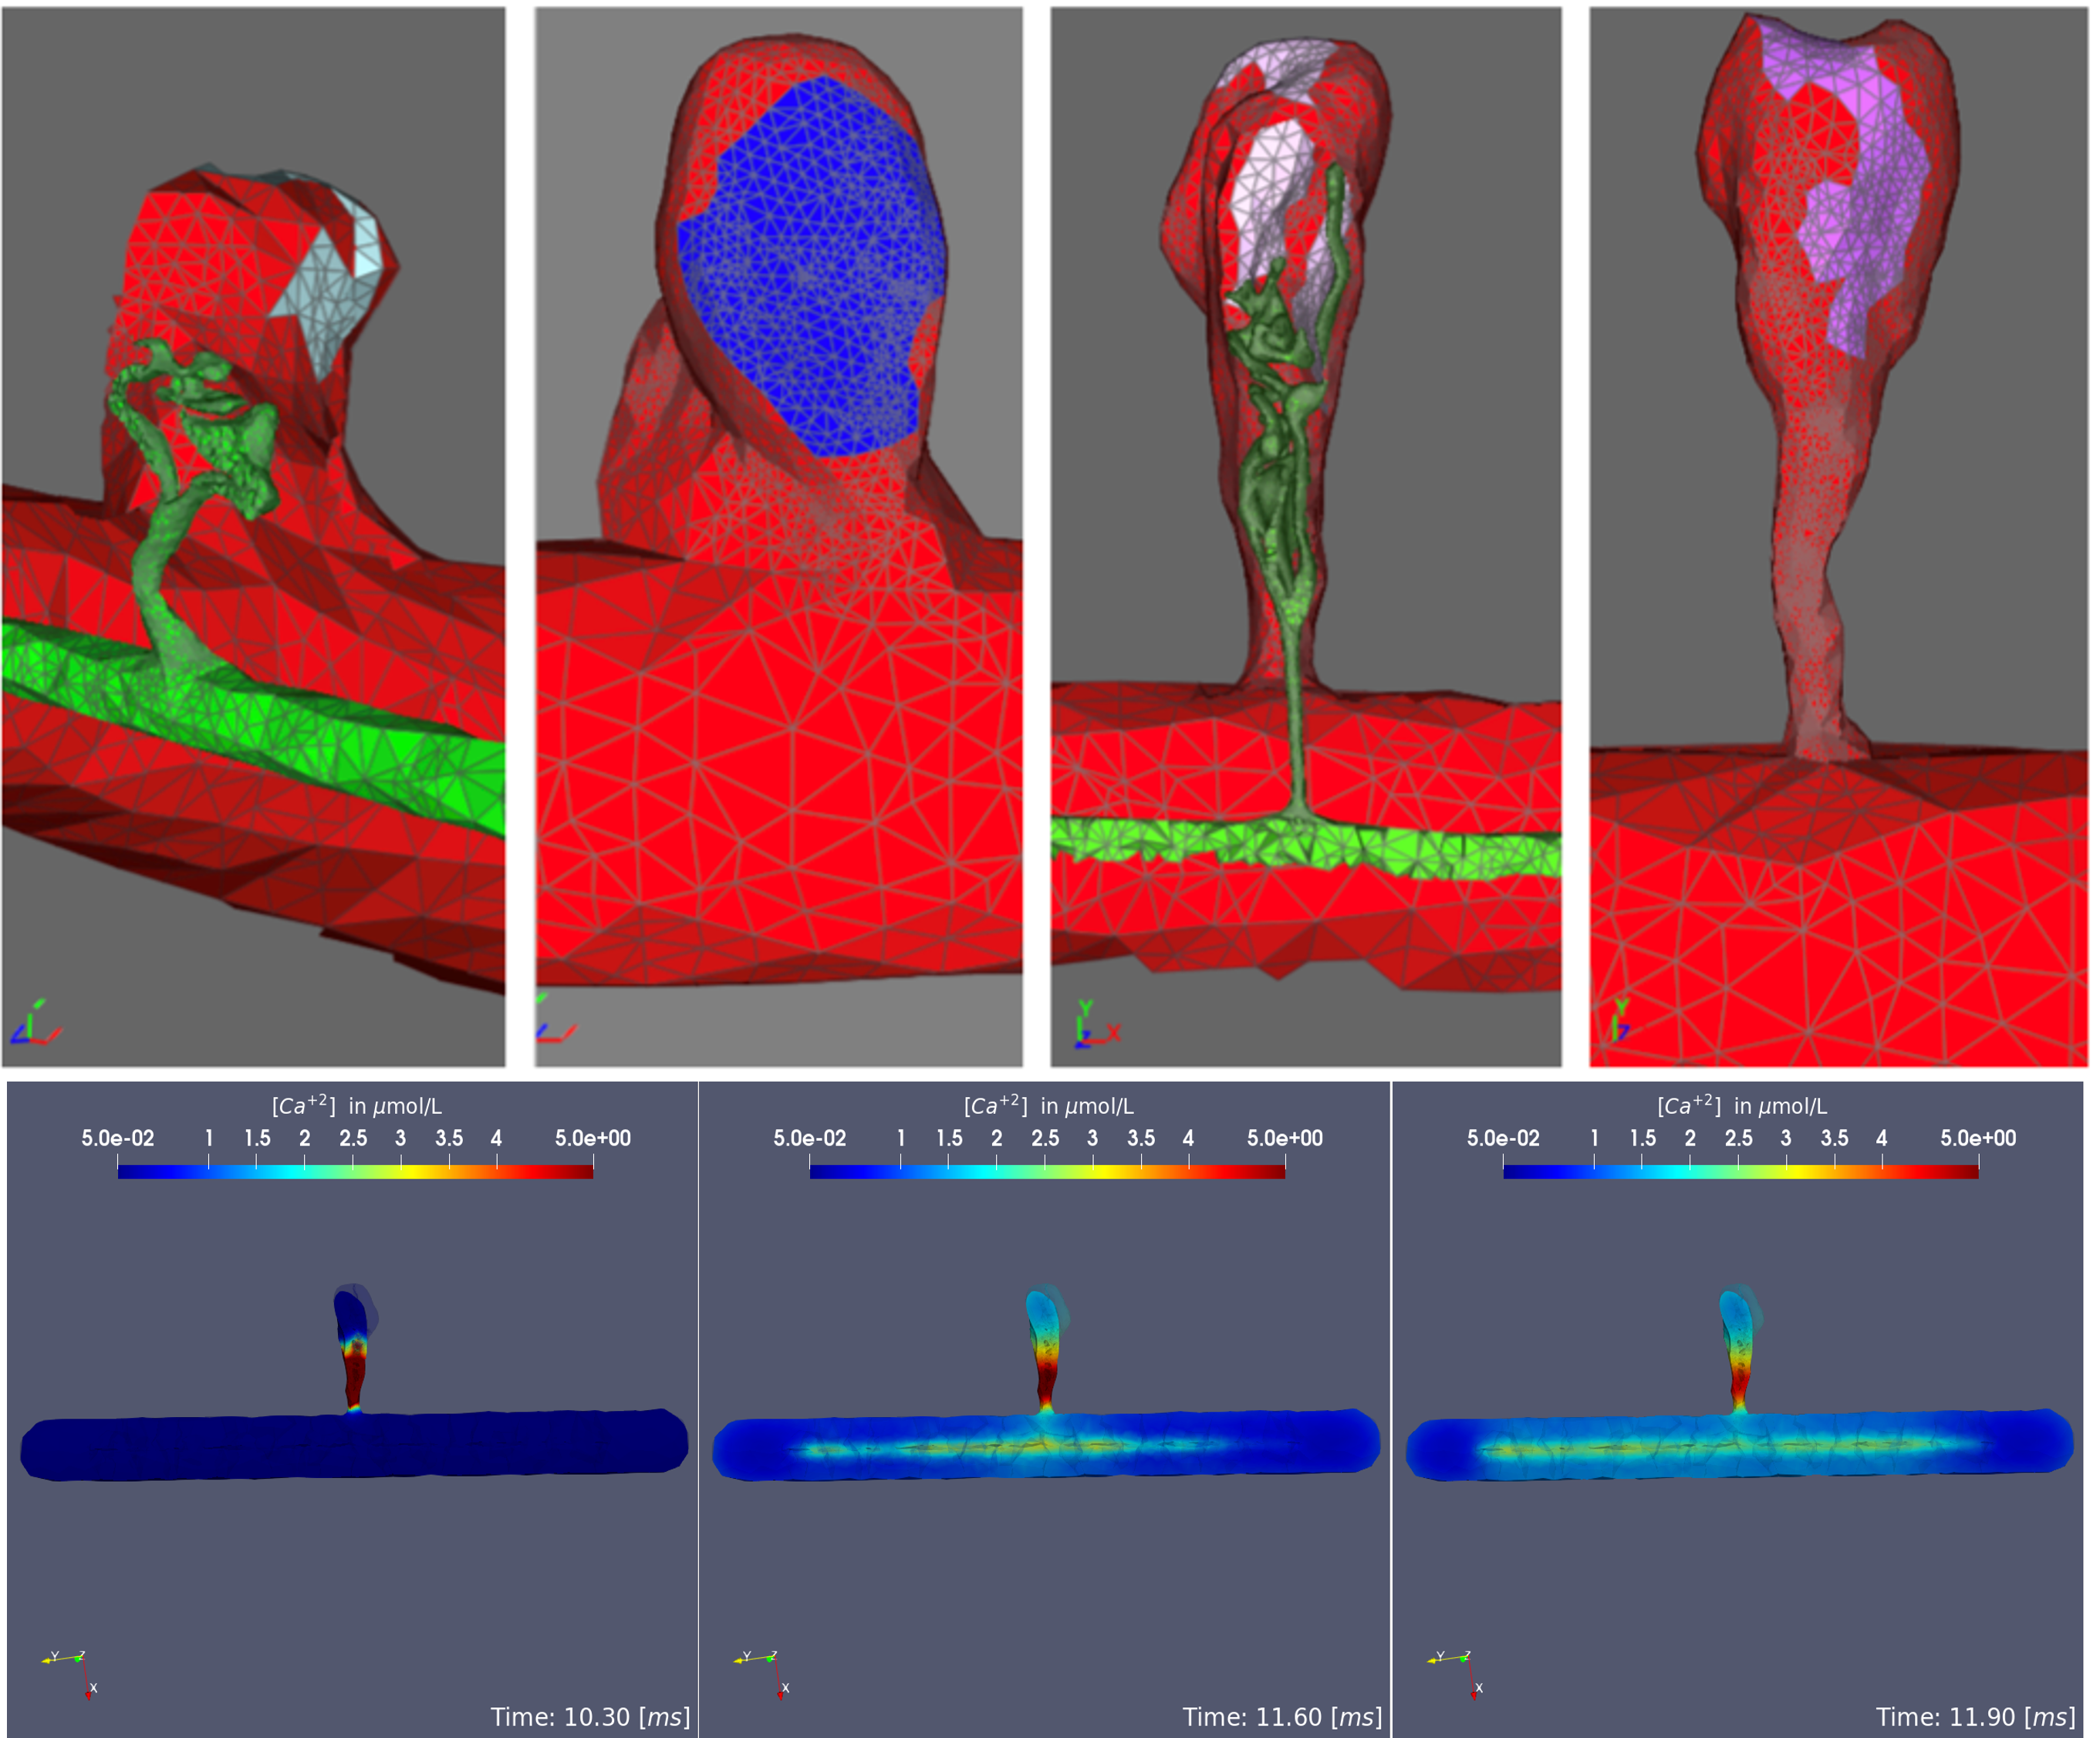
\includegraphics[scale=0.45]{inc/img/spine-types-simulationV2.png}
\caption{\textbf{Spine reconstructions and simulations:} (Top) Examples of spine reconstructions in collaboration with Dr. Vlachos (University of Freiburg, Germany). Reconstructions show variability in spine shape (red) as well as ER organization (green). (Bottom) Time sequence of a calcium simulation on reconstructed spine and dendrite geometry under VDCC activation using XSEDE resources. Color scheme: red: max. calcium concentration, blue: min. calcium concentration}
\label{fig:spine-types}
\end{framed}
%\end{wrapfigure}
\end{figure}
\noindent\textbf{Numerical method:} To computationally solve the model problem, the triangular surfaces meshes of synaptic spines, which have been generated from electron microscopy data (in collaboration with Dr. Vlachos, University of Freiburg, Germany) will be used to produce tetrahedral volume meshes using ProMesh (\cite{Reiter2012}). Using a first order finite volume method \cite{Eymard2000} the model equations are discretized on the previously generated surface and volume meshes. The nonlinear parts of the model, i.e. the Neumann boundary conditions are linearized with a Newton iteration. The resulting system of linear equations are solved by a geometric multigrid (GMG) method which is preconditioned using Bi-CGSTAB.  The GMG solve of the linear system uses 3 iterations of pre- and post- smoothing, both of which use the \textit{incomplete LU} factorization of the system matrix. We also set the \textit{SuperLU} library as the base solver for our large, sparse, nonsymmetric matrix problem. A backward Euler method is used to solve the problem in time. The proposed numerical methods are available in uG4, which will be used for all proposed computations. \\
%For numerical simulations, the four equations are
%discretized in space using a finite volumes method, \cite{Eymard2000}.
%%Control volumes are constructed as a Voronoi-like dual tesselation of the original
%%tetrahedral mesh by connecting the mid-points of edges, faces and volumes through planar facets.
%%The equations above must hold for all control volumes, giving rise to one equation per control volume.
%Time discretization is realized using a backwards Euler scheme. The described PDE problem
%should be solved by a multigrid method, \cite{Brandt1977,Fedorenko1962,Hackbusch1976,Ruge1987}. \\\\
%\textcolor{red}{Need to explain which parameters we want to vary etc.} \\\\
\noindent \textbf{Estimate of proposed simulation runs:}
Next we describe the simulations we will perform for the above project and anticipated resources. The accuracy of the simulations relies on the following: employing physiologically correct geometries, running the simulations on geometries processed through several levels of grid refinements, running the simulations with small time step size $\Delta t$ to capture the calcium dynamics in the cytosol and ER volume, and running the simulations with long end times. The studies we will perform are as follows:
\begin{itemize}
%\item[1.]\texttt{VDCC runs} -- First we will study the effects of two sources of calcium entry into the cytosol of the dendrite 
%In order to study the physiological dynamics inside the dendrite we first run simulations without ER present to establish a baseline of calcium %concentrations and general passive behavior of the calcium inside the dendrite geometry. We will run 10 simulations using a different calcium influx %value with end time $t_f=0.02\ s$ and $\Delta t = 0.5\ \mu s$ which equates to $\frac{t_f}{\Delta t} = $ 40,000 time steps.
\item[1.] \texttt{Single pulse runs} -- We will continue to run simulations with active ER having ryanodine receptors (RyR) and SERCA pumps activated. For these simulations we run a parameter sweep on the density of RyR on the ER, this will establish the critical RyR density for calcium to be released from the ER into the cytosol. {These simulations will be an expansion of our previous work (from the prior proposal) in that we will also take into account release of calcium by VDCCs. Similar to our prior work we sweep the RyR density value from 1 to 6 RyR per $\mu m^{2}$ at increments of 0.05, this amounts to 100 simulation runs, per cell.} These simulations have an end time of 20 milliseconds since coupling of calcium in the dendritic region of the cell has been observed during the first 20 milliseconds of spine activation. This simulation set has 40,000 time steps with $\Delta t = 0.5\ \mu s$.
\item[2.] \texttt{Low threshold calcium pulse runs} -- We will run studies for at least 1 second to observe the coupling effects between the spine region of the neuron and the dendrite region of the neuron for a fixed RyR density and different calcium influx pulse frequencies. These particular simulations will be performed with supercritical RyR density, each at 1 Hz, 3 Hz, 5 Hz, 10 Hz, and 20 Hz frequencies. This totals to 5 simulations, each with end time of 1 second, $\Delta t = 0.5\ \mu s$, this equates to $\frac{1.00}{0.5\times 10^{-6}}=$ 2,000,000 time steps. {We will also be setting VDCC activation by driving the VDCCs at minimum voltage gate activation, i.e. using the minimum voltage $V_m$ to induce calcium release by the VDCC.}
\item[3.] {\texttt{TMS-induced backpropagating action potential runs} -- We will also run studies for at least 0.25 seconds to observe the coupling effects between the spine region of the neuron and dendrite; with fixed RyR density (at critical) and fixed pulse frequency. In this study we will vary the voltage input at voltage dependent calcium channels (VDCCs) to determine when a stable calcium wave is propagated along the dendrite. The voltage will be varied from -70 $mV$ to 70 $mV$ at increments of 10 $mV$ (fifteen voltage levels) for each spine-dendrite geometry. This is $9\times 15 = 135$ simulations, each simulation with time step $\Delta t = 0.5\ \mu s$, this equates to $\frac{0.25}{0.5\times 10^{-6}}=$ 500,000 time steps per simulation. We will also use the data from these simulations to determine an appropriate minimum voltage to induce calcium release by VDCCs.}
\end{itemize}
We have 9 different spine-dendrite geometries that will undergo each of the above simulations. Currently, with the XSEDE trial account, we ran these simulations with 0 refinement (20,605 Degrees of Freedom -- DoFs) and 1 refinement (164,840 DoFs) on the Spine-Dendrite geometry and time step size $\Delta t =0.5\ \mu s$. In Fig.~\ref{fig:spine_dend_strongscaling2} of the \textit{performance} document we show strong scaling for a geometry \textit{without ER}. {We ran a simulation with 164,840 DoFs across 512 CPU cores with compute time of 4.69 minutes = 0.0781 hours and with simulation endtime 0.02 seconds. Therefore the number of core hours = $512\ cores \times 0.0781\ hours =  40$ core-hours. In order to capture accurate results we will process geometries with at least 1 level of refinement, with and without ER geometry present. In Table \ref{tab:sus} we indicate the anticipated compute time requirements for the sub-projects. The total number of runs is determined by $(\#\text{runs} / \text{cell})\times(\#\text{cells})$; for instance, {the \texttt{TMS runs} are 15 simulations and there are 9 cell geometries, therefore, we have $(15\ \text{runs} / \text{cell})\times(9\ \text{cells}) = 135\ \text{runs}$. 
Then the number of core-hours are computed by $(\#\text{runs})\times(\text{core-hours}/ \text{run})$; therefore, for \texttt{TMS runs} we have $(135 \ \text{runs})\times(40\ \text{core-hours}/\text{run}) = 5,400$ core-hours for a 0.02 $s$ endtime, this becomes 67,500 core-hours for 135 runs with 0.25 $s$ endtime.} Similarly for the \texttt{Single Pulse runs} we have {$(6-1)/0.05=100$ runs per cell therefore we have $100\times 40 = 4000$} core-hours per cell. For the \texttt{Low-Threshold Pulse runs} we need to take into account the number of time steps since the end time is 1 second, we have $\frac{40\ \text{core-hours}}{40000\ \text{time-steps}}\times 2000000\ \text{time-steps} = 2,000 $ core-hours per run.}
Concerning storage requirements: we have two types of data output, text files in .txt format that contain the average calcium concentration in the volume and surface regions of the cell geometry and Visualization Toolkit files (vtk) for rendering and visualizing data in 3 dimensions. We will be generating .vtk output for the \texttt{Low-Threshold Pulse runs} with active RyR \& SERCA pumps and we anticipate that each vtk file is 0.24 GiB at 1 refinement level. The \texttt{Low-Threshold Pulse} simulations run for 1 second and total 2 million time steps but we will require only 100 vtk time samples (equally distributed in time) out of the 2 million time steps. For the \texttt{Low-Threshold Pulse runs} with active RyR \& SERCA pumps we will require $\left(0.24\frac{\text{GiB}}{\text{file}}\right)\times (100\ \text{files}) \times (9\ \text{cells})\times (5\ \text{freq.})=$ \textbf{1,080 GiB} of vtk storage for all nine cells and five frequencies. {For the \texttt{TMS runs} each simulation run will produce 27,500 kB (for end time of 0.25 seconds) of data in the form of text files, at 15 runs for 9 cells this equates to $\left(27,500\frac{\text{kB}}{\text{run}}\right)\times (15\ \text{runs})\times (9\ \text{cells}) = $ 3.7 GiB.} For the RyR \& SERCA pump (\texttt{Single Pulse}) simulations, we will be performing 900 simulation runs: $\left(2750\frac{\text{kB}}{\text{run}}\right)\times (900\ \text{runs})\times (9\ \text{cells}) = $ 22.2 GiB. For the \texttt{Low-Threshold Pulse} simulations we have a run time of 1 second which equates to 137,500 kB per run; therefore, $137,500\times 15\times 9 = $ 18.6 GiB. Therefore, in total we anticipate \textbf{$3.7+22.2+18.6=$ 44.5 GiB} for text data; hence, for all spine simulations we anticipate $44.5 + 1,080 = $ 1.1 TiB. If we include ER geometry and dynamics this will incur more storage; therefore, we anticipate per month approximately \textbf{1.5 TiB} after which all data will be copied to local storage.
\subsection{Whole cell dynamics}\label{sec:whole-cell}
\textbf{The model:} While subproject \ref{sec:spine-model} focusses on the ultrastructure of individual synaptic spines, this subproject is defined on the whole cell level. The aim of this project is to study the importance of spatio-temporal synaptic activity in relaying stable calcium signals to the cell nucleus. The calcium model equations are the same as in Sec.~\ref{sec:spine-model}. The computational meshes are derived by a method developed previously in \cite{Grein2020}. The ER will be modeled as a neuron-within-neuron and can be generated alongside the surface reconstruction of a neuron. The volumetric mesh is then generated with ProMesh (\cite{Reiter2012}). The reconstruction pipeline is illustrated in Fig.~\ref{fig:anamorph}. Simulations will be run by initializing the calcium model with synapses. Synapses will be placed at distinct locations on the dendritic tree. Using standard synapse models calcium influx will be modeled as time-dependent Neumann boundary conditions. \\
\textbf{Expected outcome:} 
Calcium signals relayed to the cell nucleus by intracellular calcium waves are crucial for learning, synaptic plasticity as well as cell survival, cf. (\cite{West2002, Milner1998, Bading2000, Hardingham1997}). Neuropathologies, like Alzheimer's or ALS, impact calcium dynamics and disrupt calcium pathways (\cite{Bezprozvanny2009, Chan2009, Cheung2008, Green2008}) by loss of synapse synchronicity and/or synaptic strength.
\begin{wrapfigure}[25]{r}{0.6\textwidth}
\vspace{0pt}
\centering
\begin{framed}\raggedleft
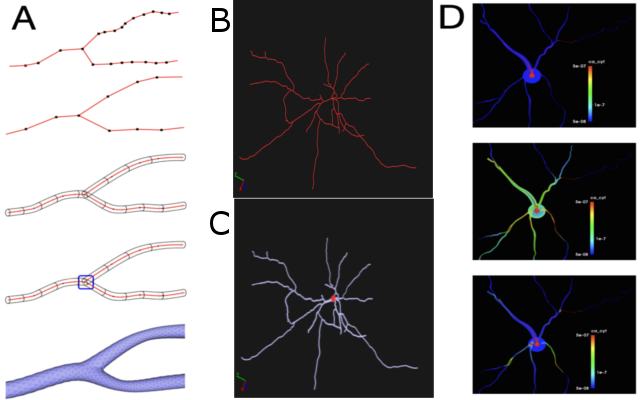
\includegraphics[scale=0.35]{inc/img/newfig.png}
\caption{\textbf{3D reconstruction pipeline}: (A) Illustration of cell surface reconstruction using graph and diameter information available from NeuroMorpho.org. The reconstruction pipeline begins with cellular graph information (B) and constructs a watertight surface triangulation (C), using the method presented in (\cite{Grein2020}). (D) Time evolution of a whole cell calcium simulation.}
\label{fig:anamorph}
\end{framed}
\end{wrapfigure}
In the previous project period we studied the necessary conditions for neurons to reliably evoke an intracellular calcium wave to transmit a signal to the cell nucleus. In particular we focussed on the effect of synaptic strength, distribution of synapses, and number of total synapses in synapse loss experiments. We hypothesized that the spatio-temporal synaptic input patterns are relevant for synapse-to-nucleus communication. To substantiate our preliminary findings, additional parameter sweeps will become necessary. In particular we intend to run simulations with a more diverse set of spatial synapse profiles and different temporal profiles, to test the influence of synapse clustering and synchronous vs. asynchronous activation on the possibility to evoke a stable or abortive intracellular calcium wave. Additionally, morphologically distinct neurons will need to be analyzed, since we recognized different synaptic stimulation patterns are required to evoke an intracellular calcium wave in different cell types.
We further hypothesize that the morphological and biophysical parameters are important for stable communication. Thus, we plan to vary relevant receptor densities of the RyR and IP\textsubscript3 receptors, activation kinetics of synapses to determine threshold parameter sets that distinguish between stable and unstable synapse-to-nucleus communication. The results of this study could 
contribute to new insight into pharmacological intervention during synapse loss, which is a major contributor in neurodegenerative diseases. \\
\textbf{Numerical method:} The numerical method for this sub-project is identical to Sec.~\ref{sec:spine-model}. \\
%We have been been developing simulation techniques
%for large-scale neuronal network simulations of networks described by graphs  (``1d'') with a
%diameter information attached to the vertices (representing idealized, cylindrical or
%cone-frustum compartments). The main results from this have been published in \cite{Breit2016}.
%We have also developed functionality to couple these large-scale 1d network simulations to fully
%resolved 3d reconstructed single-cell calcium simulations (similar to what is described in
%\cite{Grein14}). In this kind of simulation, we aim to understand the functional role of calcium
%as a messenger, taking into account the endoplasmic reticulum (ER) and a detailed model of the
%calcium dynamics including buffers as well as important endoplasmic and plasma membrane calcium
%exchange mechanisms such as the IP\textsubscript{3}R and RyR channels, voltage-dependent calcium
%channels, and sarco-/endoplasmic reticulum or plasma membrane calcium ATP-ases \cite{Breit13, Breit2018a, Breit2018b}.
%As the calcium dynamics are of special interest in the context of synaptic activity (e.g.,
%synapse-to-nucleus communication), examining a single fully resolved cell within an active
%network allows us to provide realistic synaptical inputs for the calcium simulation.
%But even with rather artificial inputs (as, e.g., given by an experimental stimulation protocol),
%single-cell calcium simulations and high-detail simulations of small regions of interest (as the
%vicinity of one or more dendritic spines) have become more and more important in our ongoing work.
%
%We would like to bring many aspects of the previous work together:
%The goal is to investigate whole-cell calcium dynamics on the basis of realistic synaptic input
%and membrane potential data from the 1d network model. In view of our basic parameter study
%about the influence of geometric parameters on calcium wave elicitation, we want to assess
%whether and under which circumstances calcium waves can occur within neurons in an active network:
%Which synaptic input patterns can lead to such waves? Can a single firing synapse cause a calcium
%signal cascade to the soma? Is the position of the synapse important (because of the
%location-specific geometry of the dendrites and ER)? Or are action potentials the only way to
%cause calcium influx into the soma (via voltage-dependent calcium channels)?
%What is the role of back-propagating action potentials? Do they significantly affect the local
%(synaptic) or even global calcium levels?
%Investigating these kinds of questions in simulations has been a long-standing goal of our
%research with implications for learning and cell survival. In past efforts a grid generation pipeline was developed with the
%goal in mind to reconstruct arbitrary cells from the \textit{Neuromorpho.org} database \cite{Ascoli2007}
%for the DMSG project and create a multigrid hiearchy. Existing tools, cf. \cite{Moerschel2017}, generated base levels too
%fine grained and thus not suitable for HPC solvers. A new ansatz was made by
%using spline data and grid generation tools from \ug which use point-diameter data.
%Volume meshes are generated efficiently by grid generation algorithms for constrained
%Delaunay triangulation \cite{Shewchuk2002, Si2005}. Based on these recent advances
%this sub-project aims to investigate by systematic parameter studies the calcium
%dynamics using the PNP model in the reconstructed cells on the sub-cellular level.
\noindent \textbf{Estimate of proposed simulation runs:} 
To study the cellular calcium dynamics from synapses to the cell nucleus, three computational setups will be used. Representative computational meshes, which will be used in the
studies outlined below and used in the strong and weak scaling benchmarks have roughly 451,485 DoFs (see Tab. \ref{tab:speedup_whole_cell}, \ref{tab:speedup_whole_cell_strong}) with run times of roughly 5 minutes for 1,000 time step on 3,074 processors.

\begin{enumerate}
\item \texttt{Variation of location of synaptic stimulation regions} -- We will use 10 representative cells from morphologically distinct regions from the NeuroMorpho.org database and generate the 3D cell and ER geometries using the approach outlined above. The number of synapses determined in the previous study which reliably triggers a calcium wave will be placed on the dendrites of neurons and we will determine whether or not stable calcium waves can be triggered by varying the dendrite diameters. For the dendrite diameter a small, medium and large endoplasmic reticulum will be considered.
For these simulation setups a simulation time of $1$ second is necessary to track calcium waves through the entire neuron. With a timestep of $0.1$ ms and 3 possible endoplasmic reticulum sizes this will amount to $3 \times 10 \times \frac{1,000}{0.1} = 300,000$ time steps for one specific synaptic stimulation pattern. We will need to address whether distribution patterns can impact wave generation in different brain regions. To address the question how spatial variation of synaptic stimulation will affect calcium waves, 5 distribution patterns will be tested: homogeneously distributed synapses 1) close to soma, 2) on distal dendrites, 3) on proximal dendrites, and clustered synapses (non-homogeneous) 4) on distal dendrites, and 5) proximal dendrites. In total $3 \times 10 \times \frac{1,000}{0.1} = 300,000$ time steps will be necessary. Using the benchmark data above, this yields $\frac{300,000}{1,000} \times \frac{5}{60} \times 3,072 = 76,800$ core hours.

\item \texttt{Variation of synaptic activation strength} -- Using the same 10 neurons we will vary receptor densities for IP\textsubscript3 receptors and RyRs to determine the conditions under which stable synapse-to-nucleus calcium communication is observed. 
For this study a simulation time of $2$ seconds is necessary. We will test 3 settings: Low, intermediate and high receptor densities. Thus, in total we expect $3 \times 10 \times \frac{2,000}{0.1} = 600,000$ time steps, which yields $\frac{600,000}{1,000} \times \frac{5}{60} \times 3,072 = 153,600$ core hours.
\end{enumerate}
\begin{enumerate}[resume]

\item \texttt{Synapse synchronicity} -- We will employ 10 representative cells to study the effect of synapse synchronicity on synapse-to-nucleus calcium communication. For this we subdivide the parameter space into a no synchronicity, 50\% synchronicity and full synaptic synchronicity. Synaptic synchronicity is known to be important for generating enough calcium influx to trigger calcium waves, important for communication in neurons from the distal to the proximal regions. From prior studies we know that abortive waves can be reliably detected within 1 s of simulation, thus when setting our time step to $0.1$ ms to resolve action potentials, $10,000$ time steps are required for one neuron. In total, for 10 neurons with 3 states and 10,000 time steps for each simulation a total of $3 \times 10 \times \frac{1,000}{0.1} = 300,000$ time steps is required. Using the above benchmark data yields $\frac{300,000}{1,000} \times \frac{5}{60} \times 3,072 = 76,800$ core hours.
\end{enumerate}
For a summary of representative simulation runs, see Table \ref{tab:sus} with 
anticipated compute time (core-h / SUs) requirements for this sub-project. Storage requirement for one VTK file is roughly 1 $MiB$ per time step. This yields, for all three studies, a total of 1.2 $TiB$.  
\subsection{Summary}
The resources required for the two projects outlined in Sec.~\ref{sec:spine-model} and \ref{sec:whole-cell} are summarized in Tab. \ref{tab:sus}. The graduate student James Rosado will be conducting all runs related to Sec.~\ref{sec:spine-model} and Stephan Grein will be responsible for all runs for Sec.~\ref{sec:whole-cell}. The postdoc Qingguang Guan and PI Queisser will support and advise efforts in both projects. \\
All participants in the project will have access to a shared file in which an estimated demand for compute time for the following project month can be submitted. James Rosado will coordinate the internal distribution of compute time for the subsequent month by weighing the individual demand against milestone deadlines, demand for conference contributions, theses finalizations and other constraints. Thus, contingent overflow as well as monthly over-demand can be minimized.

%\begin{ganttchart}[vgrid, hgrid, bar/.style={fill=blue!50},
%                    y unit chart = 0.4cm, y unit title = 0.4cm, title height=1,
%                    bar height=0.4]{1}{12}
%  \scriptsize
%  \gantttitle{Project Month}{12} \\
%  \gantttitlelist{1,...,12}{1} \\
%  \ganttgroup{\textbf{Spine}}{1}{12} \\
%    \ganttbar[bar/.style={fill=red}]{\scriptsize \textcolor{red}{Update}}{1}{6}
%  \ganttgroup{\textbf{Whole cell}}{1}{12} \\
%    \ganttbar[bar/.style={fill=red}]{\scriptsize \textcolor{red}{Update}}{1}{6}
%\label{tab:runs}
%\end{ganttchart}
